\documentclass{beamer}

\usepackage[latin1]{inputenc}
\usepackage[ngerman]{babel}
\usepackage{setspace}
\usepackage{amssymb}
\usepackage{amsmath}
\usepackage{hyperref}
\usepackage{pgf}
\usepackage{graphicx}
\usepackage{caption}
\usepackage{animate}

\beamertemplatenavigationsymbolsempty
\author[F. Loewe]{
  \leftline{\textbf{Projektpartner}: Paul Thurner}
  \leftline{\textbf{Betreuer}: Goeran Kauermann}
  \leftline{\textbf{Referent}: Felix Loewe}
}
\title[Internationaler Waffenhandel]{Internationaler Waffenhandel}
\subtitle{Die Anwendung neuer Verfahren der statistischen Netzwerkanalyse}
\institute[\textbf{LMU} -- Insitut f�r Statistik]{Ludwig-Maximilians-Universit�t M�nchen \\ Institut f�r Statistik}
%\logo{\pgfimage[width=2cm,height=2cm]{lmu_logo}}
%\titlegraphic{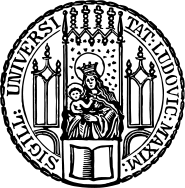
\includegraphics[width=1cm,height=1cm]{lmu_logo}}			
\date{\today}
\usetheme{Madrid}
\colorlet{beamer@blendedblue}{green!40!black}
\bibliographystyle{plain}

\begin{document}

%%%%%%%%%%%%%%%%%%%%%%%%%%%% Titel %%%%%%%%%%%%%%%%%%%%%%%%%%%%%%%
\begin{frame}
\maketitle	
\end{frame}

%%%%%%%%%%%%%%%%%%%%%%%%%%%Inhaltsverzeichnis%%%%%%%%%%%%%%%%%%%%%%%%%%%%
\begin{frame}
	\tableofcontents
\end{frame}

%%%%%%%%%%%%%%%%%%%%%%%%Einleitung%%%%%%%%%%%%%%%%%%%%%%%%
\section{Einleitung}
\begin{frame}
	\begin{center}
		\huge \textcolor[rgb]{0,0.33,0}{1 Einleitung}
	\end{center}
\end{frame}

\begin{frame}
	\frametitle{Was ist ein Netzwerk?}
	
	\begin{center}
	Netzwerk besteht aus \emph{Akteuren} und ihren \emph{Verbindungen}\\ \vspace{1cm}
	\end{center}
		
	\textbf{Anwendungsgebiete:}
	\begin{itemize}
		\item \textbf{Biologie}: DNA
		\item \textbf{Soziologie}: Freundesnetzwerk, Kollegenkreis
		\item \textbf{Politik}: internationale Beziehungen
		\item \textbf{Informatik}: Internet, Facebook, LAN
	\end{itemize}
	
\end{frame}

%%%%%%%%%%%%%%%%%%%Einf�hrung in die Graphentheorie%%%%%%%
\section{Einf�hrung in die Graphentheorie}
\begin{frame}
	\begin{center}
		\huge \textcolor[rgb]{0,0.33,0}{2 Einf�hrung in die Graphentheorie}
	\end{center}
\end{frame}

\begin{frame}
	\frametitle{Einf�hrung in die Graphentheorie}
	\textbf{Notation:}
	\begin{itemize}
		\item \textbf{$G = (V,E)$} ... ein \emph{Graph}
		\item \textbf{$V = \left\{1,...,N_V\right\}$} ... Menge der \emph{Knoten}
		\item \textbf{$E = \left\{(i,j)|i,j \in V, i\neq j\right\}$} ... Menge der \emph{Kanten}
		\item $A \in N_V \times N_V$ ... eine \emph{Nachbarschaftsmatrix} \\ \vspace{0.2cm}
	$	a_{ij} =
		\begin{cases}
		  1 \text{ , } ij \in E \\
      0 \text{ , } ij  \notin E \\
   \end{cases}
	$
	\end{itemize}
	\vfill
	\textbf{Begriffe:}
	\begin{itemize}
		\item \emph{gerichteter} vs. \emph{ungerichteter} Graph
		\item (In-/Out-) \emph{Degree}
		\item \emph{Dichte}: $den(G) = \frac{|E_G|}{N_V(N_V-1)/2}$
	\end{itemize}

\end{frame}

%%%%%%%%%%%%%%%%%%%%Datensituation%%%%%%%%%%%%%%%%%%%%%%%%
\section{Datensituation}
\begin{frame}
	\begin{center}
		\huge \textcolor[rgb]{0,0.33,0}{3 Datensituation}
	\end{center}
\end{frame}

\begin{frame}
	\frametitle{Datensituation}
	\begin{center}
		\emph{NISAT}-Datenbank (Norwegian Initiative on Small Arms Transfers) von \emph{PRIO} (Peace Research Institute Oslo)
	\end{center}
	\textbf{Kantenliste mit zus�tzlichen Variablen:}
	\begin{itemize}
		\item Correlates of War Code
		\item monet�rer Wert in US\$
		\item Waffentyp
		\item Datenquelle
		\item Jahr
	\end{itemize}
	\textbf{Dimensionen:}
	\begin{itemize}
		\item 239 L�nder
		\item 20 Jahre
		\item 109522 Waffentransaktionen
	\end{itemize}
\end{frame}

%%%%%%%%%%%%%%%%%Deskriptive Analyse%%%%%%%%%%%%%%%%%%%%%%
\section{Deskriptive Analyse}
\begin{frame}
	\begin{center}
		\huge \textcolor[rgb]{0,0.33,0}{4 Deskriptive Analyse}
	\end{center}
\end{frame}

\subsection{Netzwerkma�zahlen}
\begin{frame}
	\frametitle{Netzwerkma�zahlen}
	
	\begin{figure}
		\centering
					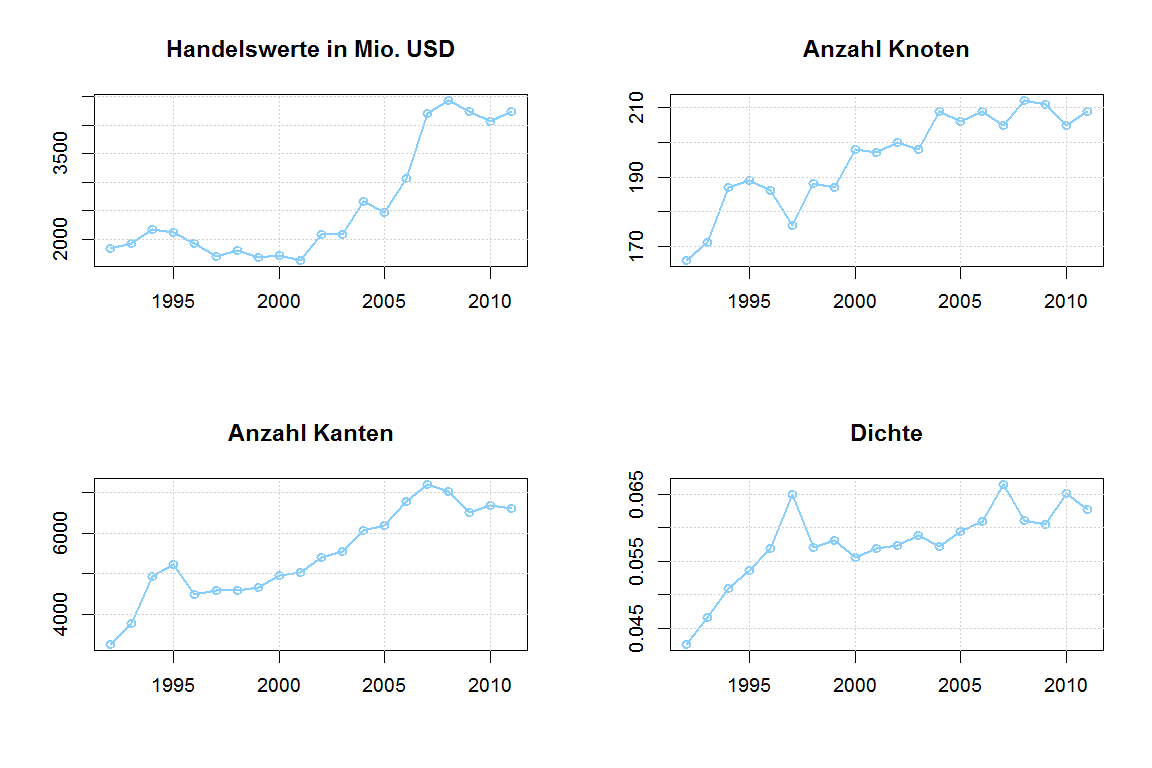
\includegraphics[width=0.8\textwidth]{Grafiken/ts_descriptives.png}
					\caption{Netzwerkma�zahlen des Kleinwaffenhandels 1992-2011}
					\label{fig:ts_descriptives}		
	\end{figure}
	
\end{frame}
\subsection{Degree-Sequenz}
\begin{frame}
	\frametitle{Degree-Sequenz}
	
	
	\begin{figure}
		\centering
			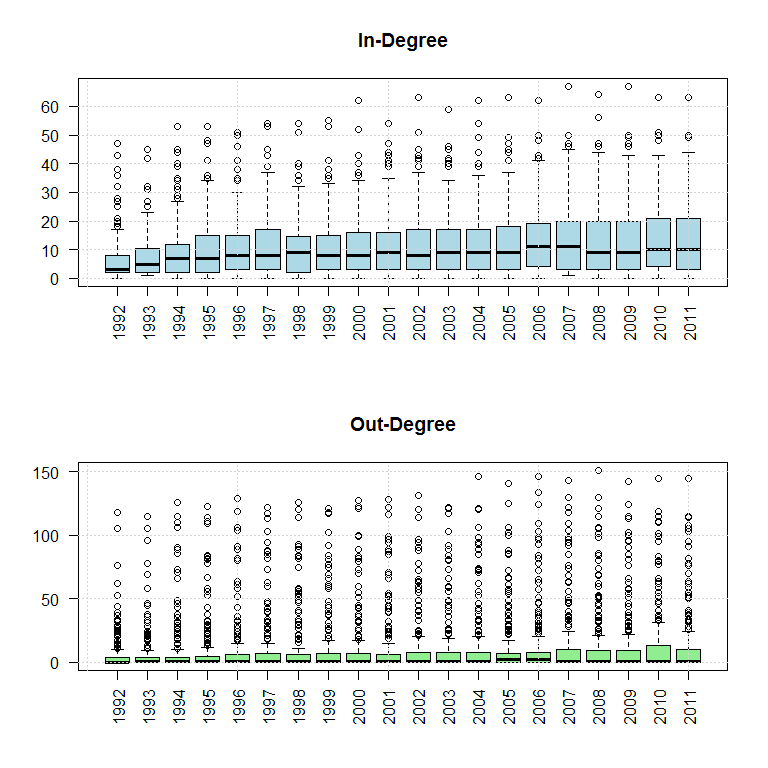
\includegraphics[width=0.7\textwidth]{Grafiken/ts_degree.png}
		\caption{In-/ Out- Degree der L�nder 1992-2011}
		\label{fig:ts_degree}
	\end{figure}
	
\end{frame}
\subsection{Zentrale Akteure}
\begin{frame}[allowframebreaks]
	\frametitle{Zentrale Akteure}
	
	\begin{table}[ht]

\centering

\begin{minipage}[t]{0.48\textwidth}
\tiny
\centering
\begin{tabular}{rlr}
  \hline
 Platz & Land & Exportvol. [Mrd.]\\ 
  \hline
1 & USA & 9.2\\ 
  2 & Italy & 7.9 \\ 
  3 & Germany & 4.6 \\ 
  4 & Brazil & 3.7 \\ 
  5 & Austria & 2.7 \\ 
  6 & United Kingdom & 2 \\ 
  7 & Belgium & 1.8 \\ 
  8 & Switzerland & 1.5 \\ 
  9 & Russia & 1.4 \\ 
  10 & Czech Republic & 1.4 \\ 
   \hline
	\end{tabular}
	\end{minipage}	
\hfill	
\begin{minipage}[t]{0.48\textwidth}	
\centering
\tiny
\begin{tabular}{rlr}
  \hline
 Platz & Land & Importvol. [Mrd.]\\ 
  \hline
1 & USA & 16\\ 
  2 & Germany & 2.3\\ 
  3 & France & 2.3\\ 
  4 & Canada & 1.9 \\ 
  5 & United Kingdom & 1.8\\  
  6 & Saudi Arabia & 1.7\\ 
  7 & Belgium & 1.2\\ 
  8 & Spain & 1.2\\ 
  9 & Australia & 1.2\\ 
  10 & Turkey & 1\\ 
   \hline
\end{tabular}
\end{minipage}
\caption{Summierte Handelswerte der Top-Exporteure und Top-Importeure des Netzwerkes von 1992 bis 2011}
\label{tab:tops}
\end{table}

\framebreak

\begin{figure}
	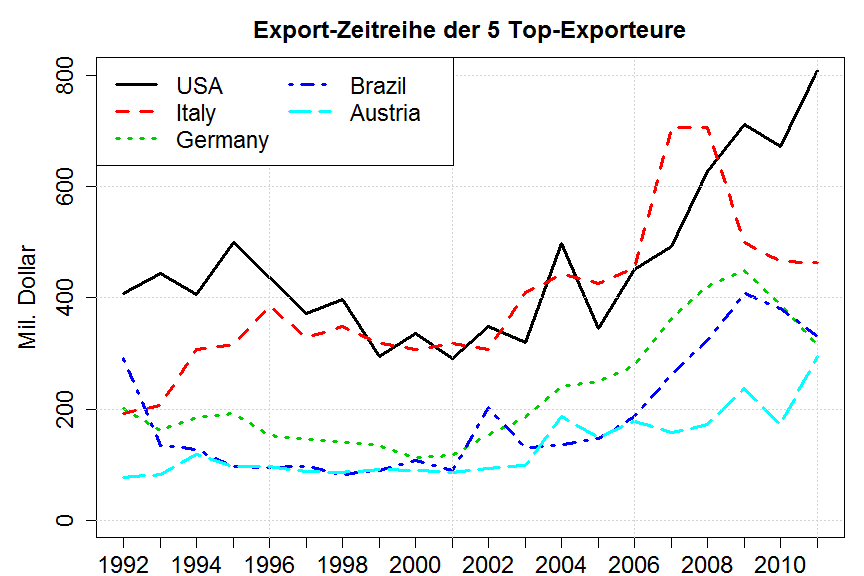
\includegraphics[width=0.65\textwidth]{Grafiken/ts_topsexp.png}
	\caption{Zeitreihen der j�hrlichen Handelswerte der Top-Exporteure von 1992 bis 2011}
	\label{fig:ts_tops}
\end{figure}

\framebreak

\begin{figure}
	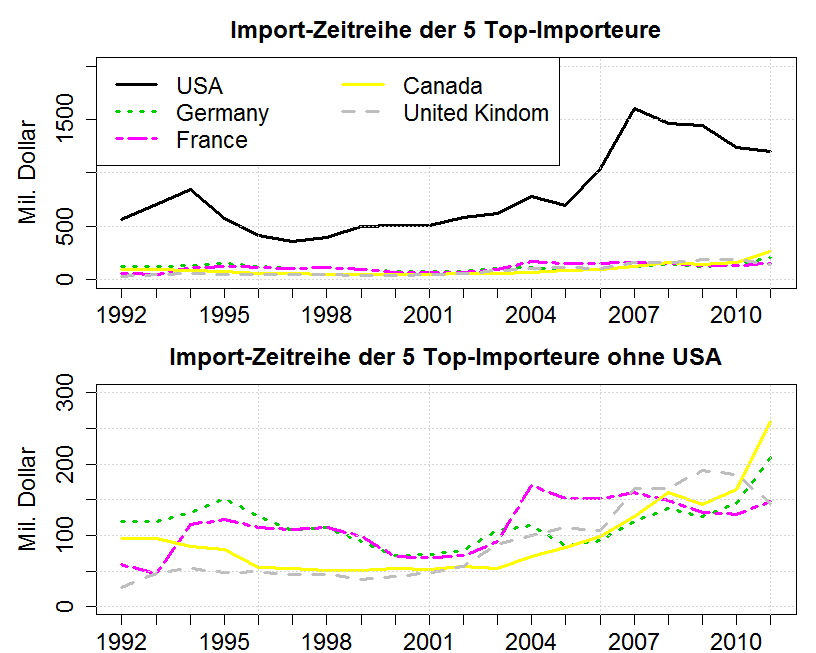
\includegraphics[width=0.65\textwidth]{Grafiken/ts_topsimp.png}
	\caption{Zeitreihen der j�hrlichen Handelswerte der Top-Importeure von 1992 bis 2011}
	\label{fig:ts_tops}
\end{figure}

\framebreak

	\begin{table}[ht]

\centering

\begin{minipage}[t]{0.48\textwidth}
\tiny
\centering
\begin{tabular}{rlr}
  \hline
 Platz & Land & Exportvol. / BIP pro Kopf\\ 
  \hline
1 & China & 114735 \\
2 & Brazil & 53225 \\
3 & Italy & 48862 \\
4 & Spain & 40822 \\
5 & Germany & 38039 \\ 
6 & Turkey & 36174 \\
7 & South Korea & 29131 \\
8 & United States & 26539 \\
9 & India & 24615 \\
10 & Austria & 23149 \\
   \hline
	\end{tabular}
	\end{minipage}	
\hfill	
\begin{minipage}[t]{0.48\textwidth}	
\centering
\tiny
\begin{tabular}{rlr}
  \hline
 Platz & Land & Importvol. / BIP pro kopf\\ 
  \hline
1 &Tanzania &54562 \\
2 &Thailand &49636\\
3 &India &32416\\
4 &Pakistan &30290\\
5 &South Korea &27208\\
6 &China &25402\\
7 &Indonesia &24268\\
8 &Kenya &22907\\
9 &Malaysia &22330\\
10 &Bukina Faso &22183\\
   \hline
\end{tabular}
\end{minipage}
\caption{Summierte Handelswerte der Top-Exporteure und Top-Importeure relativ zum BIP pro Kopf des Netzwerkes von 1992 bis 2011}
\label{tab:tops}
\end{table}

\framebreak

\begin{figure}
	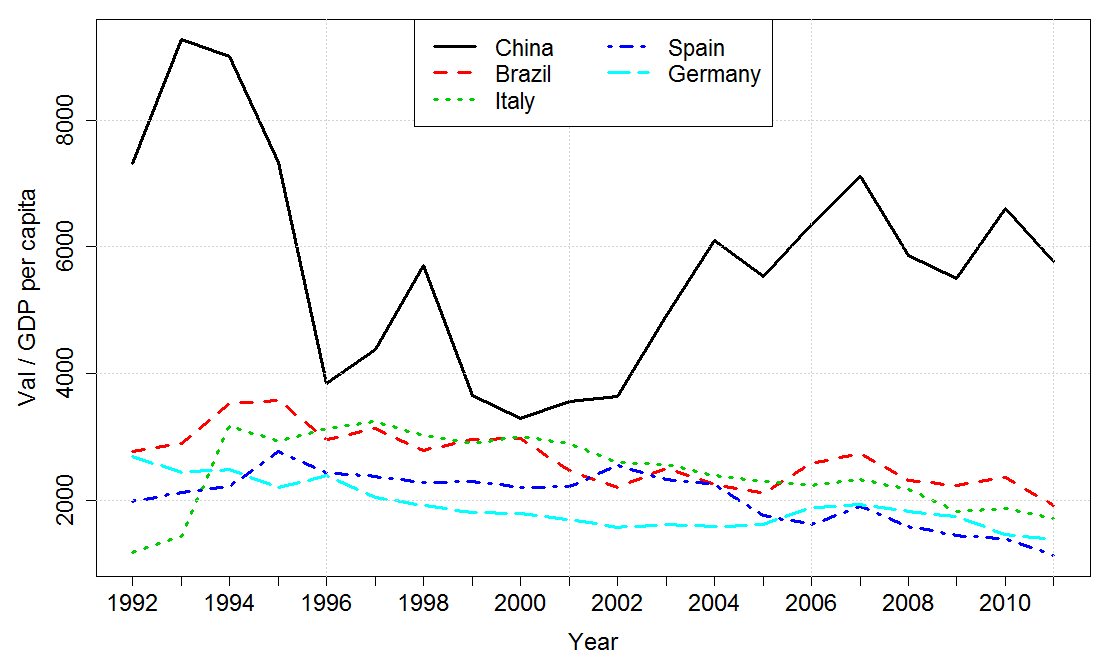
\includegraphics[width=0.75\textwidth]{Grafiken/ts_topsexprel.png}
	\caption{Zeitreihen der j�hrlichen Handelswerte der Top-Exporteure von 1992 bis 2011}
	\label{fig:ts_tops}
\end{figure}

\framebreak

\begin{figure}
	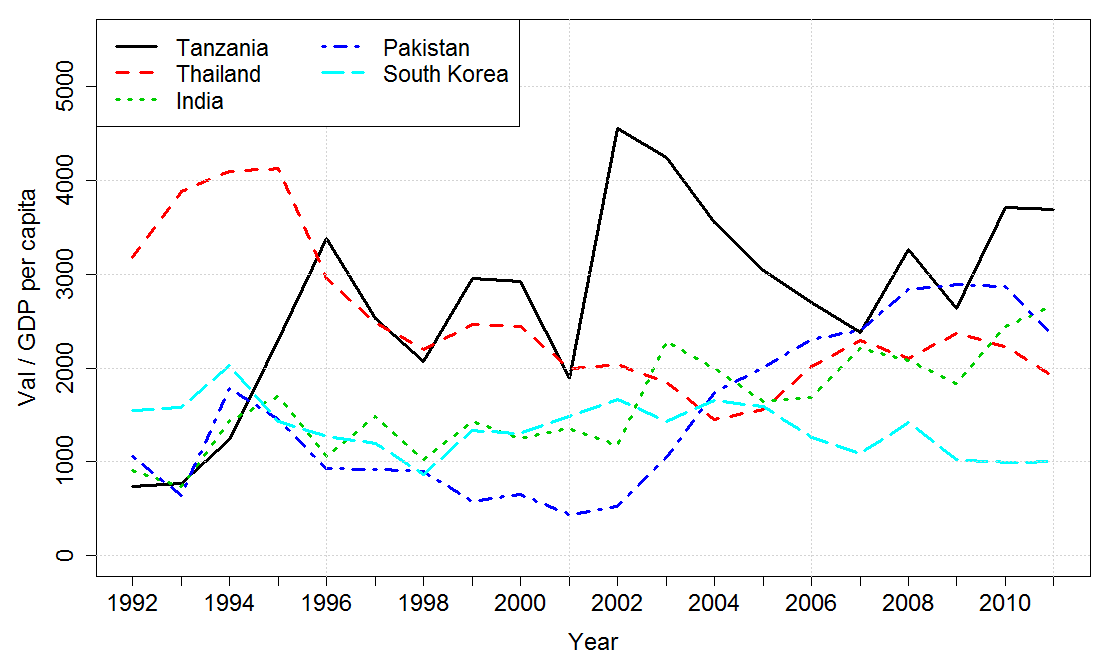
\includegraphics[width=0.75\textwidth]{Grafiken/ts_topsimprel.png}
	\caption{Zeitreihen der j�hrlichen Handelswerte der Top-Importeure von 1992 bis 2011}
	\label{fig:ts_tops}
\end{figure}

\end{frame}


\subsection{Visualisierungen}
\begin{frame}
	\frametitle{Visualisierungen}
	\begin{figure}[ht]
\centering
\animategraphics[scale=0.35, controls]{1}{Grafiken/Cont_Ani/cont}{1}{20}
\caption{Handelsstr�me zwischen den Kontinenten von 1992-2011}
\label{fig:cont}
\end{figure}
\end{frame}

%%%%%%%%%%%%%%%inferentielle Analyse%%%%%%%%%%%%%%%%%%%%
\section{Inferentielle Analyse}
\begin{frame}
	\begin{center}
		\huge \textcolor[rgb]{0,0.33,0}{5 Inferientielle Analyse}
	\end{center}
\end{frame}

\subsection{ERGM - Exponential Random Graph Model}
\begin{frame}
	\frametitle{ERGM - Exponential Random Graph Model}
	\begin{equation}
	\LARGE
	P_{\theta, \mathcal{X}}(X = x) = \frac{exp\left\{\theta^T g(x)\right\}}{\kappa(\theta, \mathcal{X})}
	\label{eq:ergm}
	\end{equation}
	mit
	\begin{itemize}
		\item $x \in \mathcal{X}$
		\item $\theta \in \Omega \subset \mathbb{R}^q$ ... Vektor der Modellparameter
		\item $g(x)$ ... q-Vektor aus Statistiken basierend auf der Nachbarschaftsmatrix $X$ \\\vspace{1cm}
		\item \textcolor[rgb]{1,0,0}{\textbf{Problem:}}  $\kappa(\theta, \mathcal{X}) = \sum_{x \in \mathcal{X}}{exp			 \left\{\theta^T g(x)\right\}}$
	\end{itemize}
\end{frame}

\subsubsection{Simulation von Zufallsgraphen}
\begin{frame}
	\frametitle{Simulation von Zufallsgraphen}
	\textbf{Simulation einer Sequenz von Graphen aus Zielverteilung $P_\theta(x)$ via Makrov Chain Monte Carlo Algorithmus:}
	\vfill
	\begin{enumerate}
	\item Beliebiges Netzwerk mit fester Knotenzahl N als Startpunkt. 
	\item Aus dem aktuellen Graphen $x^{(m-1)}$ wird ein zuf�lliges Knotenpaar $i,j$ ($i,j \in 1, ...,N$) ausgew�hlt.
	\item Vorgeschlagener Graph: $x^* = x^{(m-1)}$ bis auf $x_{ij}^{(m-1)} = 1 - x_{ij}^{(m-1)}$.
	\item Akzeptanz mit der Wahrscheinlichkeit $min\{1, \frac{P_{\theta}(x^*)}{P_{\theta}(x^{(m-1)})}\}$.
	\item Bei Akzeptanz $x^{(m)} = x^*$ und $x^{(m)} = x^{(m-1)}$ sonst.
	\item Iteration der Schritte 2 - 5.
\end{enumerate}
\begin{itemize}
	\item unabh�ngig von Startpunkt bei ausreichendem \emph{Burn In}
	\item unabh�ngige Ziehungen aus gleicher Kette durch \emph{Thinning}
\end{itemize}
\end{frame}

\subsubsection{Sch�tzung der Modellparameter}
\begin{frame}
	\frametitle{Sch�tzung der Modellparameter}
Ziel: Zentrierung der Statitiken der simulierten Netzwerke �ber denen des beobachteten Netzwerkes:

\begin{equation}
\LARGE
	E_\theta(z(X)) - z(x_{obs}) = 0
	\label{eq:1}
\end{equation}

\begin{itemize}
	\item \textbf{\textcolor[rgb]{1,0,0}{Problem:}} $E_\theta(z(X)) = \sum_{x \in \mathcal{X}}{z(x)P_\theta(x)}$
	\item \textbf{\textcolor[rgb]{0.2,0.8,0.2}{L�sung}}: \emph{Importance Sampling}
	
	\item \begin{enumerate}
		\item Ziehung einer gro�en Stichprobe von Graphen auf Basis eines vorl�ufigen Parametervektors $\tilde{\theta}$.
		\item Benutzung gewichteter Stichprobendurchschnitt der Statistiken.
		\item Erzeugen einer Sequenz von Parametern $\widetilde{\theta},\theta^{(1)}, \theta^{(2)},...,\theta^{(G)}$ durch \emph{Fisher Scoring}.
		\item Neustart mit $\theta^{(G)}$ als $\tilde{\theta}$.
	\end{enumerate}

	
\end{itemize}
\end{frame}

\subsection{Anwendung des ERGM}
\begin{frame}
	\frametitle{Anwendung des ERGM}
\end{frame}
\subsection{Vergleich mit Gro�waffenhandel}
\begin{frame}
	\frametitle{Vergleich mit Gro�waffenhandel}
\end{frame}

%%%%%%%%%%%%%%%%Fazit%%%%%%%%%%%%%%%%
\section{Fazit}
\begin{frame}
	\begin{center}
		\huge \textcolor[rgb]{0,0.33,0}{6 Fazit}
	\end{center}
\end{frame}

\begin{frame}
	\frametitle{Fazit}
\end{frame}
\end{document}